%===== TODO list =====
% Standard error or deviation for bar graph?
% Make clear that verification is a single workgoup thing
% Check and add references
% More in-depth explanation of the specification + access pattern image

\documentclass{sig-alternate-br} % Use the layout as requested by the university

%===== Used packages =====
\usepackage[utf8]{inputenc}	% Use UTF8 characters
\usepackage{url}			% Proper url in the references section
\usepackage{flushend}		% Balance the columns on the last page
\usepackage{relsize}		% Provide \mathlarger to get formula's to the correct size
\usepackage{enumitem}		% Numbered items
\usepackage{placeins}		% Used for \FloatBarrier
\usepackage{verbatim}		% Used for \begin{comment} \end{comment}
\setlist{itemsep=0pt, topsep=2pt}
\usepackage{hyperref}		% Internal references can be clicked
\pagenumbering{arabic} 	% Page numbering
% Setup captions styling
\usepackage{caption}
\captionsetup[lstlisting]{format=plain, singlelinecheck=false, margin=0pt, font={bf,footnotesize}, justification=centering}
\captionsetup[figure]{format=plain, singlelinecheck=false, margin=0pt, font={bf,footnotesize}, justification=centering, aboveskip=3pt}

%===== Code snippet styling =====
\newcommand{\code}[1]{\texttt{\small \color{inline}#1}} % \code command for inline snippets
\usepackage{listings}		% Code snippets
\usepackage{color}			% Code highlighting colors
\definecolor{dkgreen}{rgb}{0,0.6,0}
\definecolor{inline}{rgb}{0,0,0.5}
\definecolor{gray}{gray}{0.2}
\definecolor{codeText}{rgb}{0.1,0.1,0.1}
\definecolor{mauve}{rgb}{0.58,0,0.82}
\lstset{frame=tb,
  framerule=0.2pt,
  language=Java,
  aboveskip=-2mm,
  belowskip=0mm,
  showstringspaces=false,
  columns=flexible,
  basicstyle={\small\ttfamily\color{codeText}},
  numbers=left,
  numbersep=4pt,
  numberstyle=\tiny\color{gray},
  keywordstyle=\color{blue},
  commentstyle=\color{dkgreen},
  stringstyle=\color{mauve},
  breaklines=true,
  breakatwhitespace=true,
  tabsize=4
}
\lstset{language=C, escapechar=$} % Set default language to C
% Set titles for listing references
\renewcommand\lstlistingname{Algorithm}
\renewcommand\lstlistlistingname{Algorithms}
\def\lstlistingautorefname{Algorithm}
% Enable using math mode in code
\lstset{
  mathescape,         
  literate={->}{$\rightarrow$}{2}
           {ε}{$\varepsilon$}{1}
}

\begin{document}
\conferenceinfo{23$^{th}$ Twente Student Conference on IT}{June 22$^{st}$, 2015, Enschede, The Netherlands.}
\CopyrightYear{2015}

\title{Managing Big Data: GameTweets}

\numberofauthors{3}
\author{
\alignauthor Thijs Wiefferink\\
       \affaddr{University of Twente}\\
       \affaddr{P.O. Box 217, 7500AE Enschede}\\
       \affaddr{The Netherlands}\\
       \email{t.w.wiefferink@student.utwente.nl}
\alignauthor Mark Meijerink\\
       \affaddr{University of Twente}\\
       \affaddr{P.O. Box 217, 7500AE Enschede}\\
       \affaddr{The Netherlands}\\
       \email{m.j.meijerink-1@student.utwente.nl}
\alignauthor Alex Aalbertsberg\\
       \affaddr{University of Twente}\\
       \affaddr{P.O. Box 217, 7500AE Enschede}\\
       \affaddr{The Netherlands}\\
       \email{a.p.aalbertsberg@student.utwente.nl}
}
\date{\today}

\maketitle

\begin{abstract}
Abstract
\end{abstract}

\keywords{Big Data}

\section{Introduction}
This paper has been written for the course Managing Big Data at the University of Twente. The goal of this paper is to explain the preparation, execution and results of the project we performed for this course. The project required us to perform operations on a large data set, and use the results for the purpose of answering a research question. Several data sets were made available to us on the CTIT cluster at the University of Twente. 

We decided to use the Twitter data that is provided by Twiqs.nl, which contains a large part of the Dutch tweets from the period of December 2010 until November 2015. Twiqs aims to collect all tweets that are sent in The Netherlands or have a Dutch language. The tweets are filtered by language, only the tweets that are determined to be Dutch by an algorithm of Twiqs are included in the data set. Because of Twitter API limits not all tweets are collected, but estimations by Twiqs indicate that around 80\% is collected.

We wanted to research the Twitter data in the gaming area, in order to see if there is any relation between the number of tweets about a certain game (especially around the release date) and the number of copies that a game sells. Therefore the research question is as follows:
\textit{Does the number of tweets about a game relate to the number of copies sold in Europe?}

For the number of copies that a game sells, we will use the top 20 sold games from the video game sales chart on the website called VGChartz \footnote{http://www.vgchartz.com/} and filter this list to find the games that are released since 2011. The reason why we are filtering this list from the year 2011 onward is because the Twitter data also spans the period from 2011 until now. The filtered and ordered list on sales in Europe can be found in Table \ref{resultNumbers}. This list will be used during this research.

To get some first impressions about the data, we have used the web interface of Twiqs to search through the Twitter data. We have searched for ‘witcher’ (which is supposed to catch the game ‘The Witcher 3’) in the time period of January 1st, 2015 until December 31st, 2015 to see if we could find the release date. Twiqs searched in 288480444 tweets with this term and time period, and found 12032 tweets. The results show a clear peak around the end of May, which corresponds to the release date of May 19th, 2015. We also searched for ‘battlefield’, ‘fifa 15’ and ‘minecraft’ to get some more examples of game data. Out of our examples we can conclude that we can find enough tweets to find something meaningful.
\begin{figure}[!ht]
	\centering
		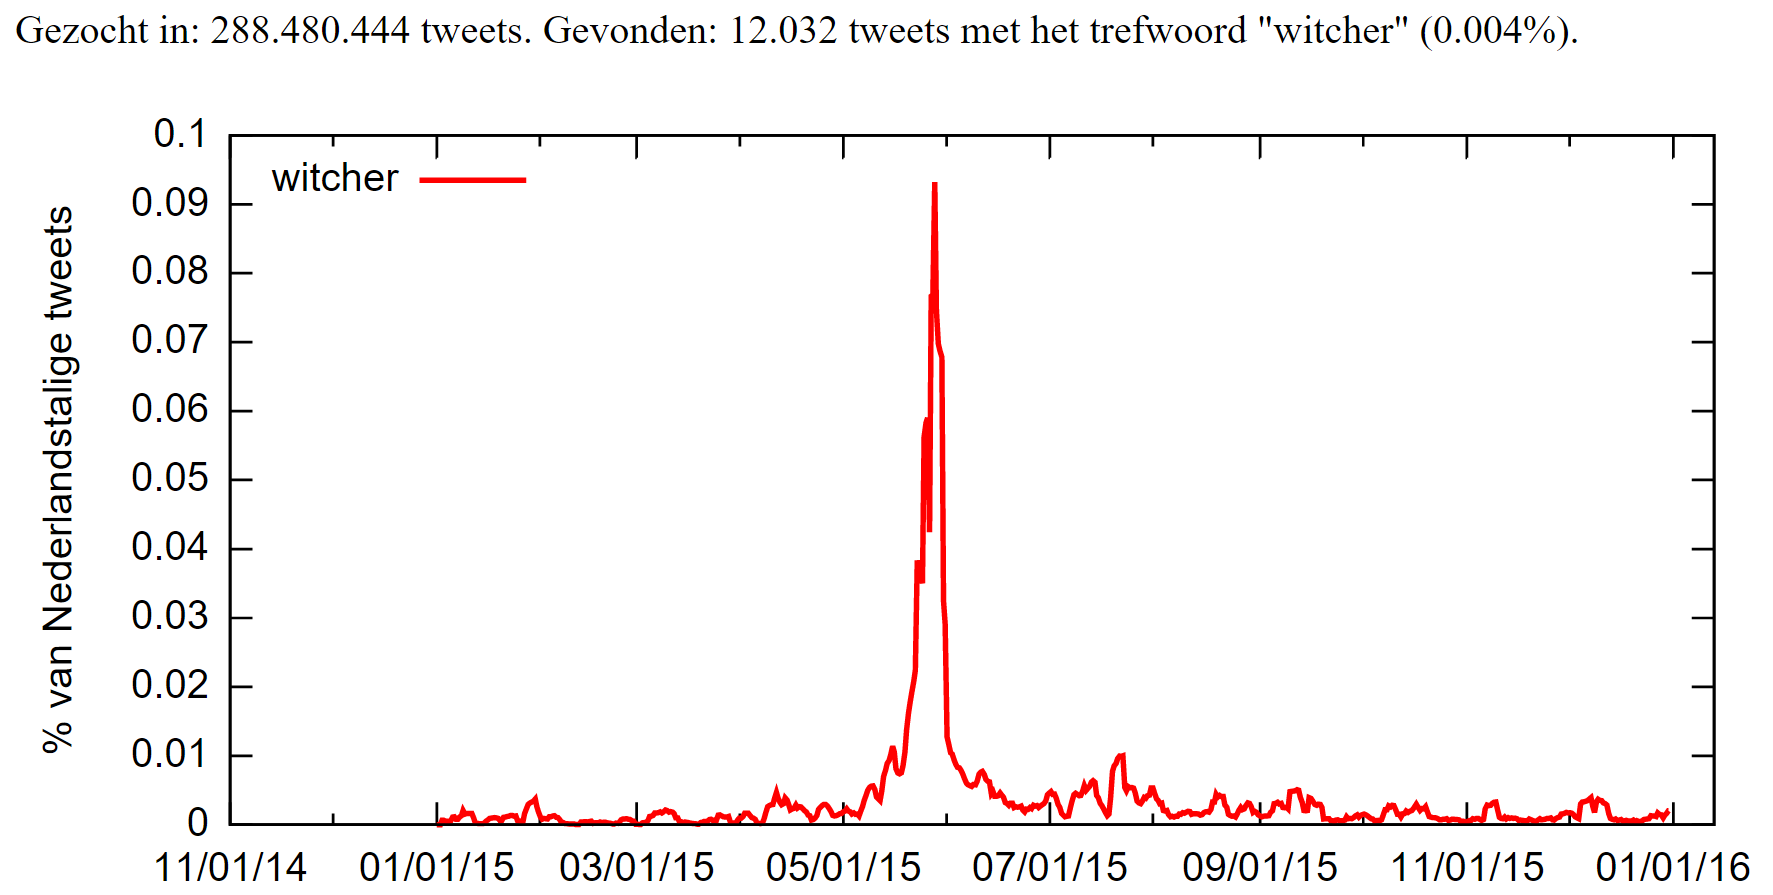
\includegraphics[width=0.476\textwidth]{twiqswitcher}
	\caption{Search on Twiqs.nl for ‘witcher’ in the period of January 2015 until December 2015.}
\end{figure}
\subsection{Need}
The results of the research will confirm or deny that there is a relation between the amount of copies that were sold and the number of tweets about the game in the release year. This relation would be useful for game publishers, game developers, game review sites and customers. For example, if there exists such a relation, then the amount of tweets that are sent at the time of release could potentially be an indicator for the estimated amount of copies that will be sold for the game. This data could be useful for publishers and developers, as it will show them the amount of excitement and interest that is being displayed for their game upon release.
\subsection{Task}
With use of MapReduce we will search in all available tweets and count the number of tweets that are about a certain game. These counts will include time data so that grouping can be used on a certain scale to get a good graph for the number of tweets related to time. It will probably make sense to group data per day. 
\subsection{Preprocessing}
The following operations will be performed on the tweet text and search terms before using them:
convert to lowercase;
remove all punctuation;
remove all whitespace characters.
These operations will ensure that we need just a few variations of the search terms, and that the search results are a lot more consistent. Using the lowercase versions makes sense because we do not want to search for each casing, and changing to lowercase does not introduce any (or at least an unnoticeable number) false positives. Removing punctuation also helps, official review sites will often use official names like \textit{Call of Duty: Advanced Warfare}, but customers will likely not use punctuation in this way, so the special characters from these need to be removed so that they match the search terms. Removing whitespace is possible because having the words of a game name directly after each other does not make any existing word, so it is not likely to appear in a tweet that is not referring to the game.
\subsection{Further steps}
A next step would be to determine the list of games from the Twitter data itself, instead of searching with a predefined list. Game names could be scanned for by checking for the words before/after the word ‘game’. Then this game list could be used as input for the initial program to calculate the score for each game. Challenges for automatically determining the list of games would be finding the names, and keeping the list clean. This is hard because normally game names are not mentioned with a certain term in front or after it, so it is not trivial to find these.
\subsection{Expected results}
The result of this research will consist of comparisons between the amount of tweets that have been created about a game and its sales records. The results of the amount of tweets will be visualized as a graph and will usually show a peak in the amount of tweets sent around the time of a game’s release date. The answer to our research question depends on whether there is a correlation between the amount of tweets that have been sent and the amount of copies that were sold. As an end result, we will deliver a ranked top 20 list of the chosen games, and compare this to the list based on sales numbers.



\section{Materials and Methods}
The MapReduce code has been implemented in such way that the result has less data-noise and have as much game-related-tweets as possible. To achieve this, the data first is preprocessed. All tweets are converted to lowercase-text with only numbers and letters. This gives the opportunity to use less search terms, because all spaces and other special characters in the game names are filtered out the tweets. 


The 20 top sold games in Europe since 2011 and their search terms are put in a HashMap, so that the tweets of all games can find in a single MapReduce job.
  
\section{Results}
With the materials and methods that have been described, we have executed a MapReduce job on the CTIT cluster. This job has counted the tweets that have been sent about a game on every day from December 2010 until November 2015. These tweet counts have been processed and their results have been made visible using highcharts, one of which can be seen below. We chose to use highcharts, because they contain some handy functions such as zooming in on a particular time period. The full results for all of the games in the top 20 can be found on the website that we have created. \footnote{http://wiefferink.me/GameTweets}.

\begin{figure}[!ht]
	\centering
	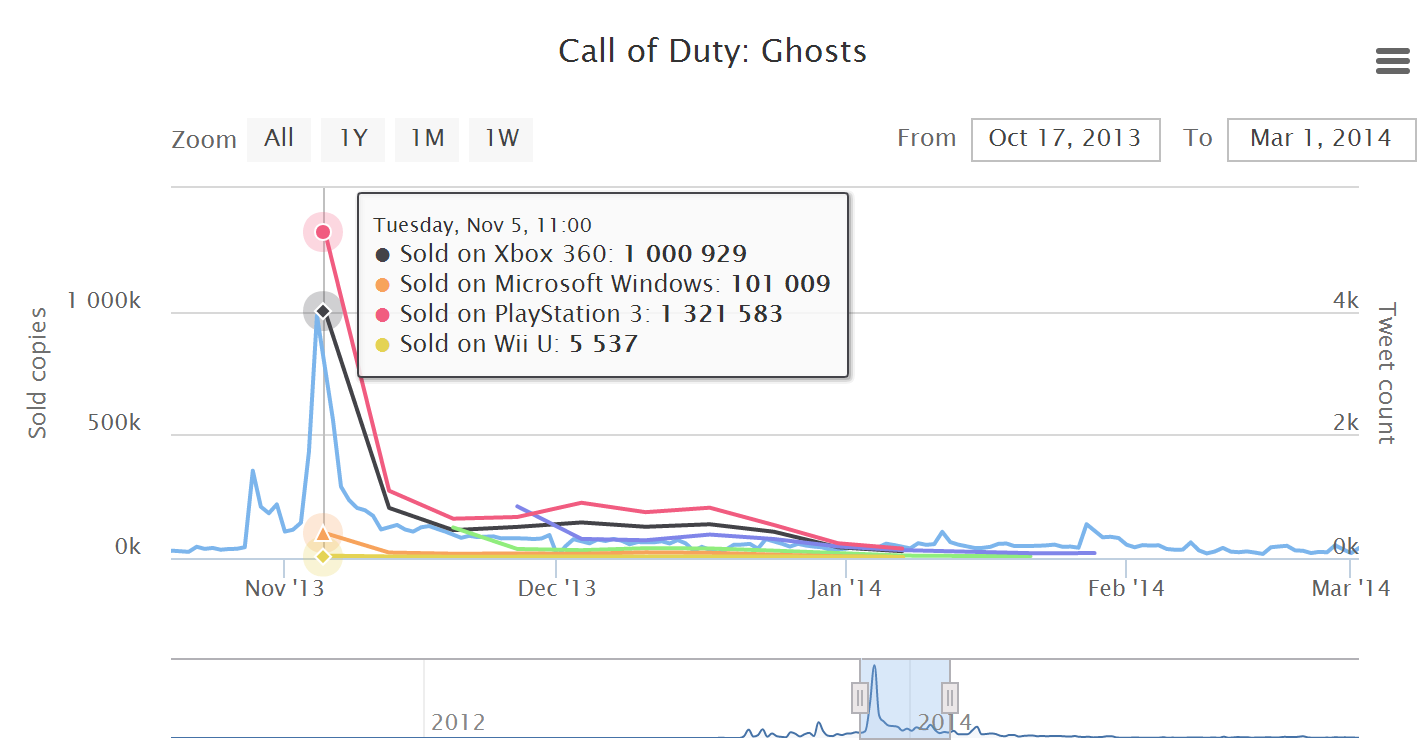
\includegraphics[width=0.46\textwidth]{highchart-ghosts}
	\caption{Highchart for the game Call of Duty: Ghosts (zoomed in around the release date).}
	\label{highchartghosts}
\end{figure}

This image \ref{highchartghosts} represents the amount of tweets that were sent daily about the game Call of Duty: Ghosts.  The release date for the game was November 5th, 2013.

The main result of this research was to check for a correlation between the amount of tweets that were sent about a certain game, and its position in the sales charts. For the purpose of checking for such a correlation, we decided to take the Twitter results and the sales charts, and create a list that contains both for all of the games. This list has been included in this report as \ref{resultNumbers}.
\section{Discussion}
The MapReduce job took about 8 hours to complete on the cluster, so this meant that we could not perform this job often. To prevent us from needing to do this, we started by running our MapReduce code on smaller data sets, such as the number of tweets in one or two months. This allowed us to remove bugs from the code quickly, and test the data processing for the website before we ran the job on the complete data set.

There are several things that may have influenced the results, such as:
\begin{itemize}
	\item We may not have been able to consider all tweets referring to specific games. Some tweets may only contain the name of the franchise, as people will not always spell out the game's full name. (FIFA 15 may become just FIFA, and Grand Theft Auto V may become just GTA).
	\item Unfortunately, the collection of tweets does not span the full 100\% of Dutch tweets that were sent in the time period. The estimate is that the data set contains approximately 40\% of all the tweets \cite{sangDealingWithBigData}.
	\item The time period during which tweets have been collected spans from December 16th, 2010 until November 5th, 2015. Because some of the games were released either before or right before the end of this time period, we may not have all tweets that refer to this game around its release.
	\item Something else we have noticed, is that the number of tweets drops at around May 10th, 2014. This may be due to an error or an adaptation on Twiqs' side.
	\item Instead of only the number of tweets, also favorites and retweets of the tweet that mentions a game might be used. This might give a better estimation about the popularity of the game.
\end{itemize}
\section{Conclusion}
Conclusion
\section{Appendices}
\subsection{Results}
The results can be found in Table \ref{resultNumbers}.


\newpage % Column balancer
\bibliographystyle{abbrv}
\bibliography{GameTweets}
\newpage % Fixes weird alignment of last reference

\end{document}
